\section{Generative Model}

In this section we first review LDA and then review a model known as the doubly hierarchical Pitman-Yor process model (DHPYPLM) \cite{Wood2009a}. We will conclude by proposing a novel combination of the two models to infer latent domains and a set of hierarchical Pitman-Yor process language models (HPYPLM's) \cite{Teh2006a} in a set of documents.

\subsection{Latent Dirichlet Allocation}

LDA \cite{Blei2003} is a mixed membership model for documents.  If we characterize a topic as a multinomial distribution over words then the generative process is that each document is a bag of words, where each word is drawn from one component of the mixture over topics. The generative model for $J$ documents containing $T$ possible topics is written as 

\begin{eqnarray}
\phi_t | \beta  &\sim& \textrm{Dir}_{|\Sigma|}(\beta)  \hspace{.7cm} t = 1,\ldots,T \nonumber \\
\psi_j | \alpha &\sim& \textrm{Dir}_T(\alpha) \hspace{.85cm} j = 1,\ldots, J\nonumber \\
z_{ij} | \psi_j &\sim& \textrm{Mult}(\psi_j) \hspace{.7cm} i = 1,\ldots, N_j \nonumber \\
w_{ij} | \phi_{z_{ij}} &\sim& \textrm{Mult}(\phi_{z_{ij}}) \hspace{.5cm} i = 1,\ldots, N_j 
\end{eqnarray}

\noindent where $w_{ij}$ is the $i^{th}$ word in the $j^{th}$ document, $N_j$ is the number of words in document $j$, and $\Sigma$ is the set of possible words in the language. \footnote{It is assumed for this discussion that $| \Sigma| < \infty$} The notation $\textrm{Dir}_T(\alpha)$ means a dirichlet distribution over multinomial distributions with $T$ components such that each parameter is $\frac{\alpha}{T}$.  To generate word $i$ in document $j$, $w_{ij}$, a topic indicator $z_{ij}$ is drawn from the document specific mixture $\psi_j$ and $w_{ij}$ is drawn from the appropriate topic $\phi_{z_{ij}}$. 

Estimation of the model can been performed using a collapsed Gibbs sampler \cite{Griffiths2004}.  In this case the parameters $\{ \phi_t \}$ and $\{ \psi_j \}$ are integrated out and each topic label $z_{ij}$ is sampled from the conditional distribution $p(z_{ij} | w_{ij}, \mathbf{z}_{-ij}, \mathbf{w}_{-ij})$, where $\bf{z_{-ij}}$ is the vector of topic assignments for all words other than $w_{ij}$ and $\bf{w_{-ij}}$ is the corpus of words other than $w_{ij}$.

\subsection{Doubly-Hierarchical Pitman-Yor Process Language Model}

The DHPYPLM is a nonparametric Bayesian model that ties together individual HPYPLM's. Sharing of statistical strength between language models is achieved through a process known as the Graphical Pitman-Yor Process (GPYP) \cite{Wood2009a}.  Because the DHPYPLM builds upon the HPYPLM, we first describe the HPYPLM.

The HPYPLM is a non-parametric Bayesian hierarchical model specifying that each word is generated from a distribution specific to the context ${\bf u}$ in which the word appears.  For this discussion the context of a given word, $w_i$, is  defined as the ordered sequence of the $n-1$ words preceding it, $[w_{i - (n-1)}, w_{i-(n-2)}, \ldots, w_{i-1}]$.  Context specific distributions $\G_{\bu}$ are tied together through the hierarchical structure

\begin{eqnarray}
\G_{[]}| c_0, d_0, \mathcal{U} &\sim& \PY(c_0, d_0, \mathcal{U}) \nonumber \\
\G_\bu | c_{|\bu|}, d_{|\bu|}, \G_{\pi (\bu)} &\sim&  \nonumber \\
& & \hspace{-1cm} \PY( c_{|\bu|}, d_{|\bu|},  \G_{\pi (\bu)})  \label{eqn:hpyplm}
\end{eqnarray}

where $\bu \in \Sigma^{n-1}$, $\Sigma$ is the set of possible words, and $\pi(\bu)$ is the context obtained by removing the most distant word from the context $\bu$.  The notation $\G \sim \PY(c,d,\G_0)$ indicates that $\G$ is a random distribution following a Pitman-Yor process distribution with concentration parameter $c$, discount parameter $d$, and base distribution $\G_0$.

Use of a HPYPLM assumes a single language model responsible for generating all text.  However, there are instances in which the assumption of a universal language model is inappropriate \cite{Rosenfeld2000}.  In \cite{Wood2009a} they develop the GPYP, a fully Bayesian coupling of HYPYLM's. The resulting model can be understood as a generative model with a latent, general HPYPLM serving as a common prior for each of several domain specific HPYPLM's.  The common language model is referred to as latent because no data generated directly from the latent model is ever observed.  Typical of Bayesian hierarchical models, the language model for each domain reflects properties of the general HPYPLM while still capturing differences in the language structure of each domain.  

In the DHPYPLM, the latent language model is a HPYPLM, as specified by Equation~\ref{eqn:hpyplm}.  If $G^\LA_\bu$ is the distribution over words given the context $\bu$ in the latent language model, then for each domain $\D$,  the domain specific model is

\begin{eqnarray}
\G^\D_{[]} &\sim& \PY(c^\D_0, d^\D_0,\G^\LA_{[]}) \nonumber \\
\G^\D_\bu &\sim& \PY(c^\D_{|\bu|}, c^\D_{|\bu|}, \lambda^\D_{|\bu|}\G^\D_{\pi(\bu)} \nonumber \\
&& \hspace{-1cm} + (1-\lambda^\D_{|\bu|})\G^\LA_\bu))  \hspace{.2cm} \forall \bu \in \Sigma^{n-1}, 0 \leq \lambda^\D_{|\bu|} \leq 1. \nonumber
\end{eqnarray}

Each distribution described is actually a conditional distribution, but the conditioning bars have been left off to reduce clutter in the notation.  Explicitly, the distribution of $\G^\D_{[]}$ is conditioned on $c^\D_0, d^\D_0,$ and $\G^\LA_{[]}$, etc.  Note that the base distribution of each Pitman-Yor process for each $\G^\D_\bu$ is a mixture of distributions: the first is the distribution in the same domain given a context shortened by one word while the second is the distribution given the context $\bu$ in the latent language model. Priors are also placed on all $\lambda^\D_{|\bu|}$ parameters, \cite{Wood2009a} use

$$\lambda^\D_{|\bu|} \sim \PY(\alpha_{|\bu|}, \delta_{|\bu|}, \textrm{Unif}(0,1))  \hspace{.5cm} \forall \D.$$

Using this prior ties together the $\lambda_{|\bu|}$ parameters across different domains $\D$ under a common prior.

The generative process specified by the  DHPYPLM can be equivalently written in a collapsed representation known as the multi-floor Chinese restaurant franchise (MFCRF) \cite{Wood2009a}.  Using the MFCRF \cite{Wood2009a} show that estimation can be performed using a collapsed Gibbs sampler.

\subsection{A Latent Domain Hierarchical Language Model (\ourmodel)}

We suggest that documents are likely to include language from from multiple domains and that language structure varies across domains. This hypothesis indicates that an appropriate language model must infer latent domains and a set of language models to explain the language structure within a set of documents.

We consider a model which combines the two models previously discussed.  Each document is modeled as a mixture of domains.  To generate the $i^{th}$ word in document $j$, $w_{ij}$, a domain is chosen from the document specific mixture.  Given the domain $z_{ij}$ and the context $\bu$ in which $w_{ij}$ is observed, $w_{ij}$ is drawn from the HPYPLM specific to to domain $z_{ij}$.  The domain specific language models are tied together through a GPYP.  Formally the generative model is

\begin{eqnarray}
\psi_j  &\sim& \textrm{Dir}(\alpha) \nonumber\\
z_{ij}  &\sim& \textrm{Mult}(\psi_j) \nonumber\\
\lambda^{z_{ij}}_{|\bu|} &\sim& \PY(\alpha_{|\bu|}, \delta_{|\bu|}, \textrm{Unif}(0,1)) \nonumber \\
\G^{z_{ij}}_{[]} &\sim& \PY(c^{ z_{ij}}_0, d^{ z_{ij}}_0,\G^\LA_{[]}) \nonumber \\
\G^{ z_{ij}}_\bu &\sim& \PY(c^{ z_{ij}}_{|\bu|}, d^{ z_{ij}}_{|\bu|}, \lambda^{ z_{ij}}_{|\bu|}\G^{ z_{ij}}_{\pi(\bu)} \nonumber \\
&& \hspace{1.5cm} + (1-\lambda^{ z_{ij}}_{|\bu|})\G^\LA_\bu)) \nonumber \\ 
w_{ij}|\G^{z_{ij}}_\bu  &\sim& \G^{z_{ij}}_\bu \nonumber.
\end{eqnarray}

\begin{figure}[t] 
	\begin{center}
		\scalebox{.2}{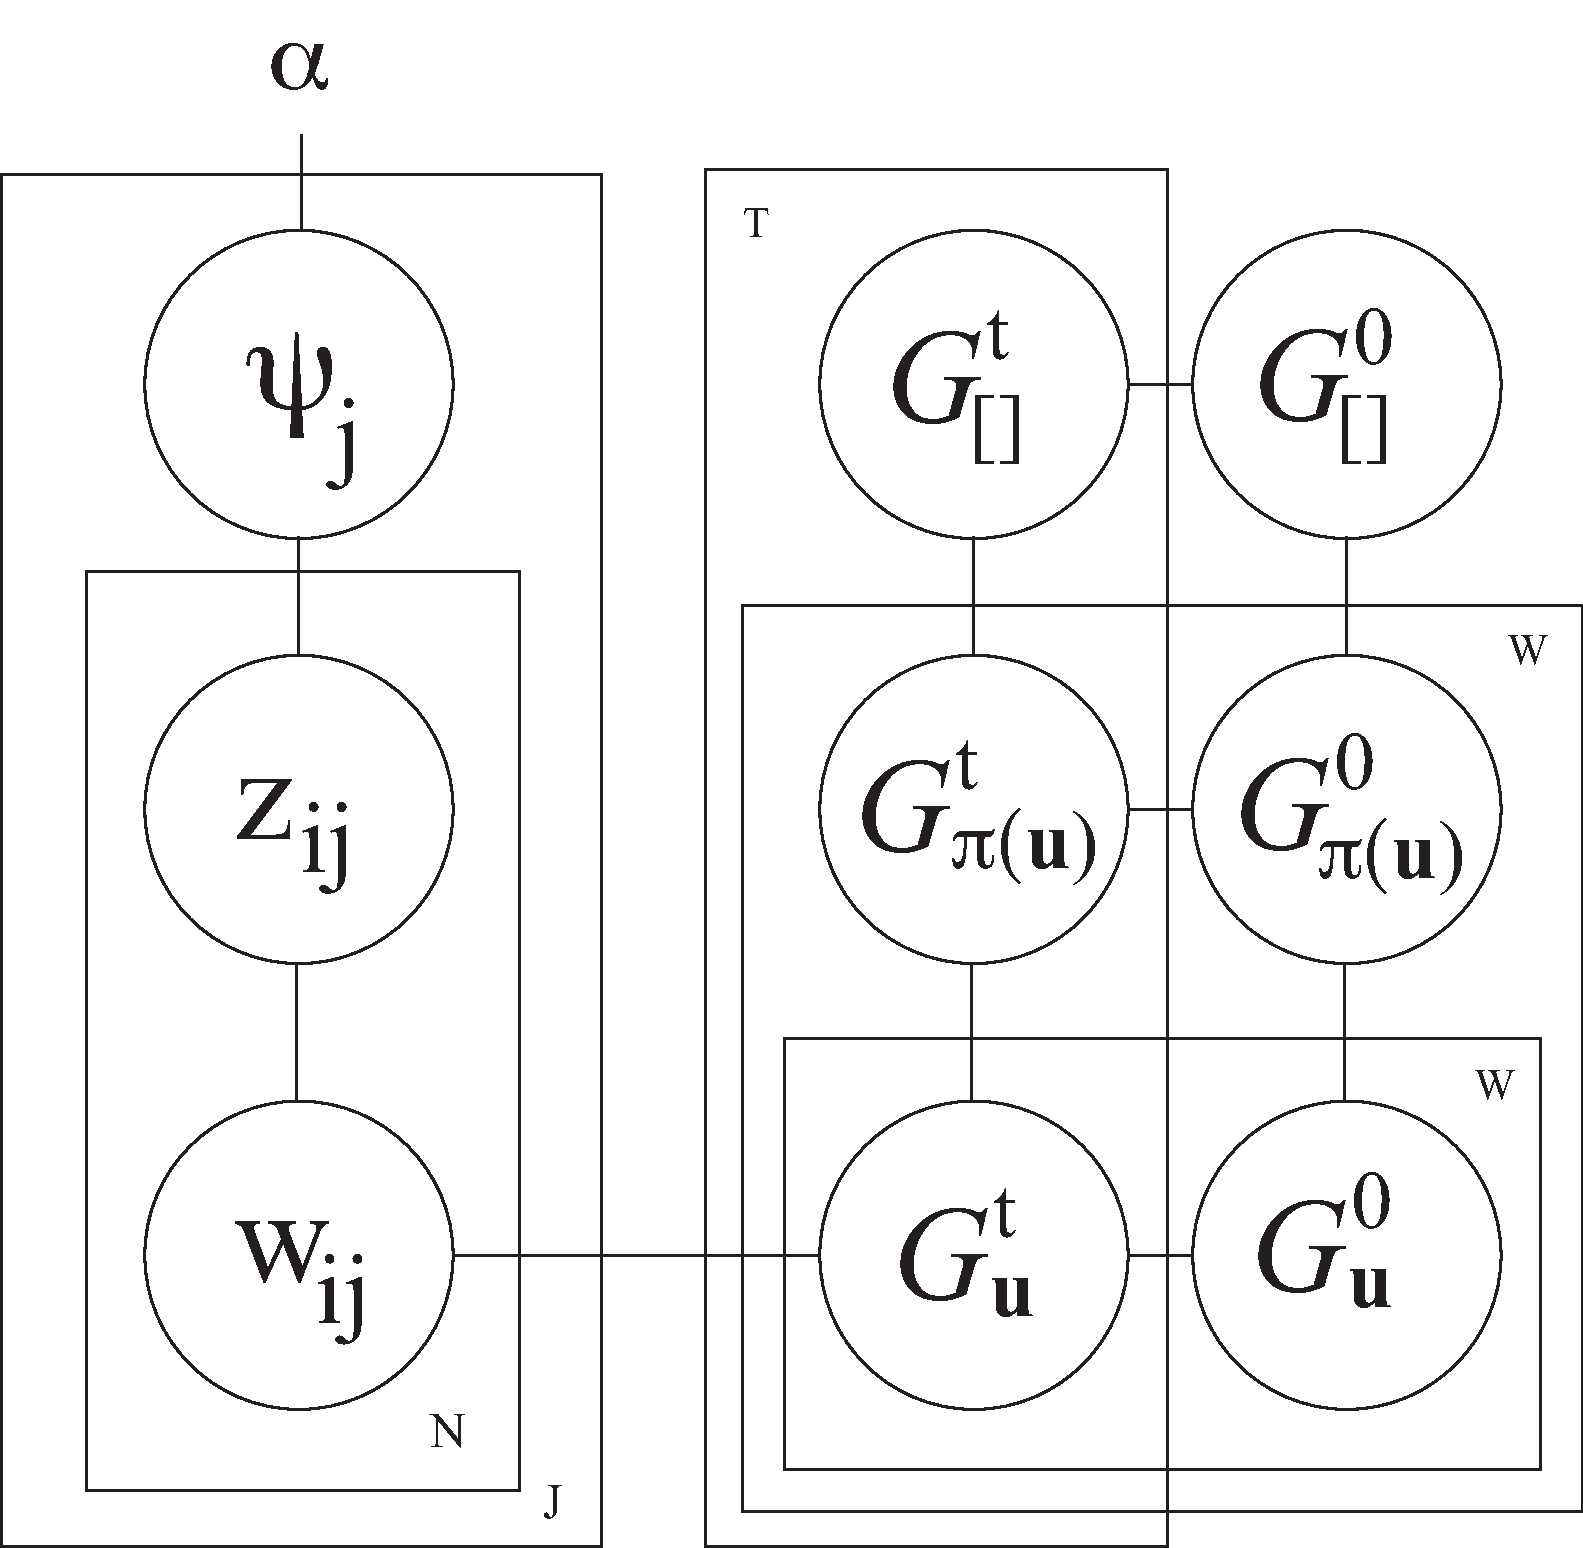
\includegraphics{LDA-DHPYPLM2.pdf}} % [clip=true, viewport= 1in 1in 9in 9in]
		\caption{Graphical Model}
		\label{fig:graphicalmodel}
	\end{center} 
\end{figure} 

The conditioning variables have again been omitted for clarity, but are implicit in the definition.  Figure~\ref{fig:graphicalmodel} shows the graphical model for the proposed model.

